%!TEX root = document.tex

% Note: activity SAGs can go beyond friends.

%In this section we evaluate the correlation between the conditional
%entropy and size of groups, pages and favourites.

Now we analyse the informativeness of Activity Social Affinity
Features (ASAFs) by looking at the correlation between the size and
type of groups, pages and favourites.

Fig~\ref{Fig3} provides scatter plots of conditional
entropies and logistic regression weights vs. activity group 
size.\footnote{Here the size of a {\em group}, {\em page} and {\em favourite}
is the number of total users in the activity group.  For {\em pages}
and {\em favorites} this is the total number of Facebook users,
whether or not they are in the App users' ego network, while for {\em
groups} only the number of users in the App users' ego network is
visible to our app.}  Both plots show that small activity groups
\emph{can} be highly predictive (low conditional entropy or
weights that deviate extremely from zero) whereas large groups are
\emph{rarely} predictive.

In Fig~\ref{Fig4} we plot the average conditional entropy of the top
10\% of features cumulative up to the size of the activity group given
on the x-axis.
%; this allows us to determine the marginal contribution
%of larger groups to the average conditional entropy as they 
%are incrementally added in.  
This graph distinctly shows that the
small sizes of groups, pages and favourites have low average
conditional entropy that transitions sharply to a higher average 
at about 50 for groups and $10^{5}$ for pages/favourites.

%{\bf TODO: make this consistent with earlier discussion regarding persistence,
%temporally sychronized.}

We also analyse predictiveness of favourites by categories obtained
from the Facebook API in Fig~\ref{Fig5}.
We can see that categories like movie, books, or movies with
``long-tail'' (less widely popular) content may not be
the most predictive on average, but %%% HERE
least popular content in the 
is often most informative.  On the contrary, generic affinities
(e.g. interests) and those with a smaller number of choices
(e.g. sports or fav-teams) tend to be less predictive since they
represent less specialised interests than the long tail of music,
book, or movie preferences.

These observations of Fig~\ref{Fig5} are also reiterated by the
examples provided in Table~\ref{table:fav_examples} where
uninformative favourites tend to have a broad appeal whereas
informative favourites generally appear much more specialised.  This
also reinforces the point that not all SAGs are predictive, but some
are very predictive and it is important to learn which SAGs are
informative rather than nai\"{v}ly aggregate their content, where on
average, the features are clearly not informative.
   
%#suvash#
In Fig~\ref{fig:AccuracyVsactiveFeats} we analyse the relationship
between accuracy and number of active features i.e. features that are
true. We can see that accuracy increase as number of active features
increases but then starts to decrease sharply. This is due to the fact
that items with large number of active features are likely to be
general items, liked by wide variety of users, which makes it hard for
SAF to make correct prediction. In Fig~\ref{AccuracyVsmembership} we
can see that , in general, accuracy of SAF increases as number of
group memebership, page likes and favourites increase.  This indicates
that SAF can make better recommendation to those users who actively
express their preferences in a social network via group memebership,
page likes and favourites.
    
%While favourite teams, sports and athletes may be
%too focused to offer much predictiveness vs. the other more diverse
%categories, it is interesting that movies and music favourites
%are not very predictive on average.  This may have to do with the fact that
%these are typically ephemeral favourites that may be heavily influenced
%by popularity as opposed to true personal preference.
%\end{itemize}

%In Fig~\ref{Fig4} we plot the average conditional entropy of top
%    10\% features cumulative over the size of activity group. It
%    distinctly shows that the small sized group, pages and favourites
%    have low average conditional entropy. Furthermore, it explains
%    average conditional entropy decreases as size increases. From the
%    figure \ref{Fig4} we can infer that the group size upto 50 and
%    page/favourite size upto $10^{5}$ can be highly predictive.
%
%We also analyze predictiveness of favourites by categories in
%    Fig \ref{Fig5}. It shows that television, books, music and movies
%    are predictive whereas favourite teams, sports and athletes are
%    less predictive.
%\end{itemize}

%\TODO{add a table of top 5-10 groups/pages/favs}

\begin{table*}[t!] \centering 

{\small
\begin{tabular}{|c|c|c|c|c|}
\hline 
\multicolumn{5}{|c|}{\textbf{Median Informative Favourites by Category}}\\
\hline 
\textbf{Books} & \textbf{Movies} & \textbf{Music} & \textbf{Television} & \textbf{Interests} \\
\hline \hline
Harry Potter series&Forrest Gump&John Lennon&Futurama&Travel\\
\hline
A Song of Ice and Fire&Pretty Woman&U2&Star Trek&Music\\
\hline
Discworld&Napoleon Dynamite&AC/DC&The Trap Door&Literature\\
\hline
Hitchhiker's Guide To The Galaxy&Harry Potter&The Smashing Pumpkins&Drawn Together&Painting\\
\hline
The Hobbit&Toy Story 3&Gotye&Sherlock(Official)&Running\\
\hline
The Magician's Guild&The Godfather&The Rolling Stones&Hitchhiker's Guide to the Galaxy&Sports\\
\hline
Ranger's Apprentice&Mulan&All Axess&Buffy The Vampire Slayer&Films\\
\hline
Cosmos&How to Train Your Dragon&Steve Aoki&South Park&Genetics\\
\hline
%Foundation and Earth&The Princess Bride&Rihanna&24&Travelling\\
%\hline
%Deception Point&Watchmen&Billy Joel&The Daily Show&Internet\\
%\hline
%%%%%%
%5 point someone&Black Swan&Queens of the Stone Age&Monty Python's Flying Circus&Psychology\\
%\hline
%Freakonomics&Inception&Depeche Mode&Top Chef&Math\\
%\hline
%Alex Rider Series&Donnie Darko&Oasis&The Inbetweeners&Lambda\\
%\hline
%The Elenium&Kung Fu Panda&Justice&Firefly&Computer Science\\
%\hline
%Watchmen&American Psycho&Gorillaz&Red Dwarf&Skepticism\\
%\hline
\multicolumn{5}{c}{}\\
\hline 
\multicolumn{5}{|c|}{\textbf{Most Informative Favourites by Category}}\\
\hline
\textbf{Books} & \textbf{Movies} & \textbf{Music} & \textbf{Television} & \textbf{Interests} \\
\hline \hline
Calvin and Hobbes & Billy Madison & Avascular Necrosis & Metalocalypse & Computers\\
\hline
Tomorrow when the War Began & Team America: World Police & Tortured & Beast Wars & Texas HoldEm \\
\hline
I really like ceilings  & Pan's Labyrinth & Elysian & Hey Arnold! & Programming\\
\hline
Angels and demons  & Pirates of the Caribbean & Anno Domini & Sherlock & Economics\\
\hline
Magician  & Aladdin & Darker Half & Hey Hey It's Saturday & Martial arts\\
\hline
Digital Fortress  & Starship Troopers & Hellbringer & Neil Buchanan and Art Attack! & Graphic design\\
\hline
The Bible  & Happy Gilmore & Johnny Roadkill & Breaking Bad & Cooking\\
\hline
Interview with the Vampire  & Timon and Pumbaa & Aeon of Horus & Red vs. Blue & Klingon language\\
\hline
%The Discworld Series  & Ferris Buellers Day Off & Katabasis & Stargate Universe & Politics\\
%\hline
%The Da Vinci Code  & Peter Griffin & Bane Of Isildur & Chaser's War on Everything & Science\\
%\hline
\end{tabular}}

\caption{(top) Examples of 8 items per Favourite category near the \emph{median} conditional entropy (\emph{median informativeness}).
(bottom) Examples of top 8 items with the lowest conditional entropy
(\emph{most informative}).  A general trend is that more informative
favourite category ASAGs tend to be more specialised in appeal,
e.g. ``Avascular Necrosis'' is an informative music group favourite
--- its members tend to share common preferences --- while ``John
Lennon'' and ``U2'' have a broader audience with more diverse
preferences.
%#suvash#
Interestingly, ''Sherlock'' appears in both most and median
informative table but the median informative is an official page with
wide range of fans, whereas the most informative is a duplicate fan
page with few fans.}
\label{table:fav_examples}
\end{table*}

\eat{
\begin{table*}[tbp!]
\centering
\begin{tabular}{| >{\small}l | >{\small}r | >{\small}r |}
\hline
\textbf{Top Groups} & \textbf{Top Pages} & \textbf{Top Favourites} \\
\hline
%Heavy Metal - Australian Capital Territory & Avascular Necrosis & Avascular Necrosis \\
Heavy Metal - (city name) & Avascular Necrosis & Avascular Necrosis \\
Stephen Conroy Should Not Filter Our Internet & Assidian & Tortured \\
Silicone Stripper & Tortured & Elysian \\
Hardcore dancing is not moshing & Elysian & Anno Domini \\
%Metal bands come to Canberra cause I'm sick of... & Darker Half & Hellbringer \\
Metal bands come to (city name) cause I'm sick of... & Darker Half & Hellbringer \\
%Canberra Rock Gigs & Johnny Roadkill & Johnny Roadkill \\
(city name) Rock Gigs & Johnny Roadkill & Johnny Roadkill \\
%Let's Mosh - Canberra metal radio show - 2XX 9 & Anno Domini & Darker Half \\
Let's Mosh - (city name) metal radio show - 2XX 9 & Anno Domini & Darker Half \\
Bring Steel Panther to Australia & Billy Madison & Bane Of Isildur \\
%Canberra Death/Heavy Metal Appreciation & Hellbringer & Katabasis \\
(city name)  Death/Heavy Metal Appreciation & Hellbringer & Katabasis \\
Robert The Bruce (Band) & Metalocalypse & Aeon of Horus \\
\hline
\end{tabular}
\caption{Top 10 Groups/Pages/Favourites ranked by Conditional Entropy. The city name where our institution and many Facebook users resides is anonymized.}
\label {table:topGroupPagesFavs}
\end{table*}}

%%%%%%%%%%%%%%%%%%%%%%%%%%%%%%%%%%%%%%%%%%%%%%%%%%%%%%%%%%%%%%%%%%%%%%%%%%%
\begin{figure*}[tbp!]
\centering
\begin{tabular}{ccc}
\begin{tabular}{ccc}
\subfloat[Fig:][]{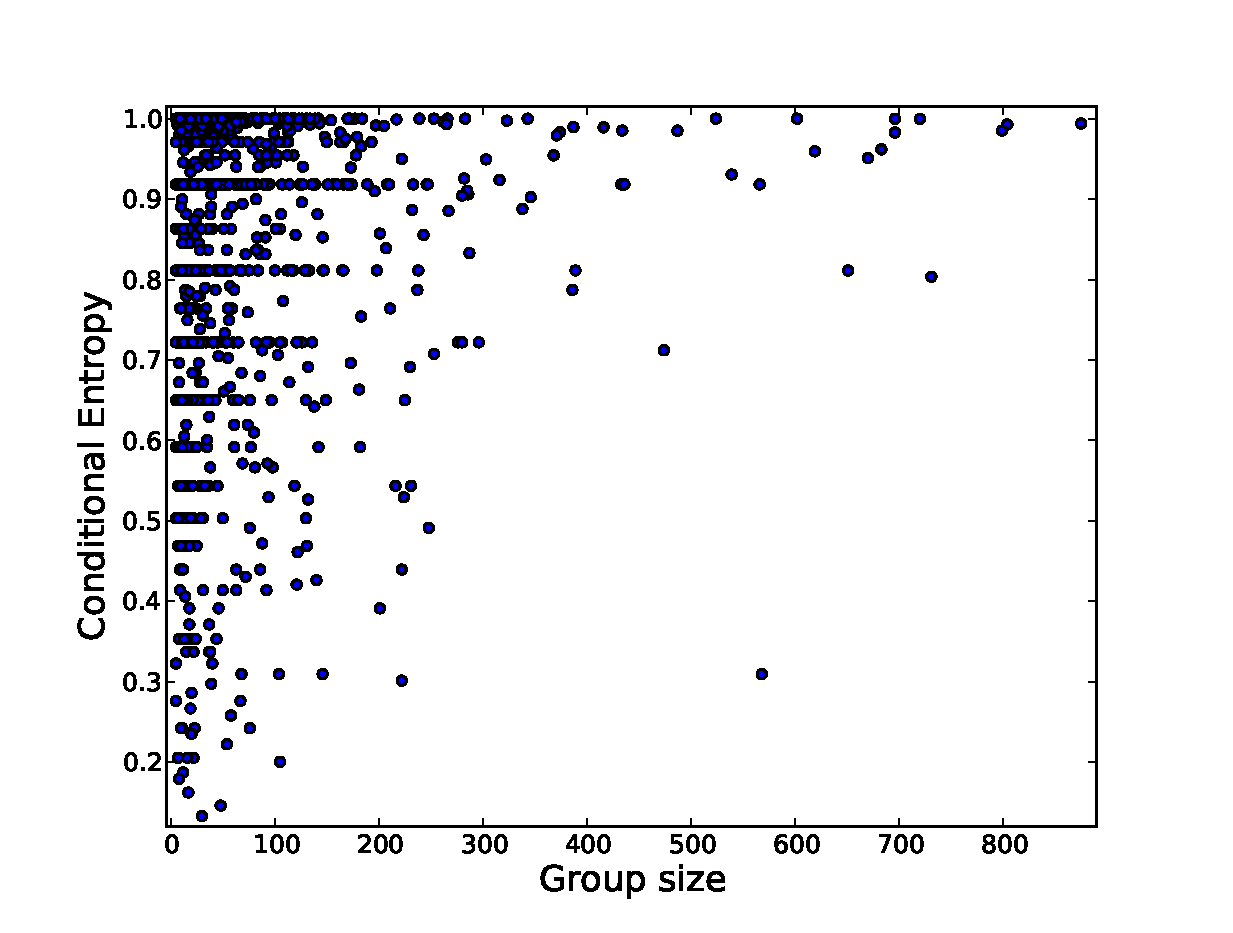
\includegraphics[width=45mm, height=35mm]{data/plots/new/CEvsGroupSize.eps}}
\subfloat[Fig:][]{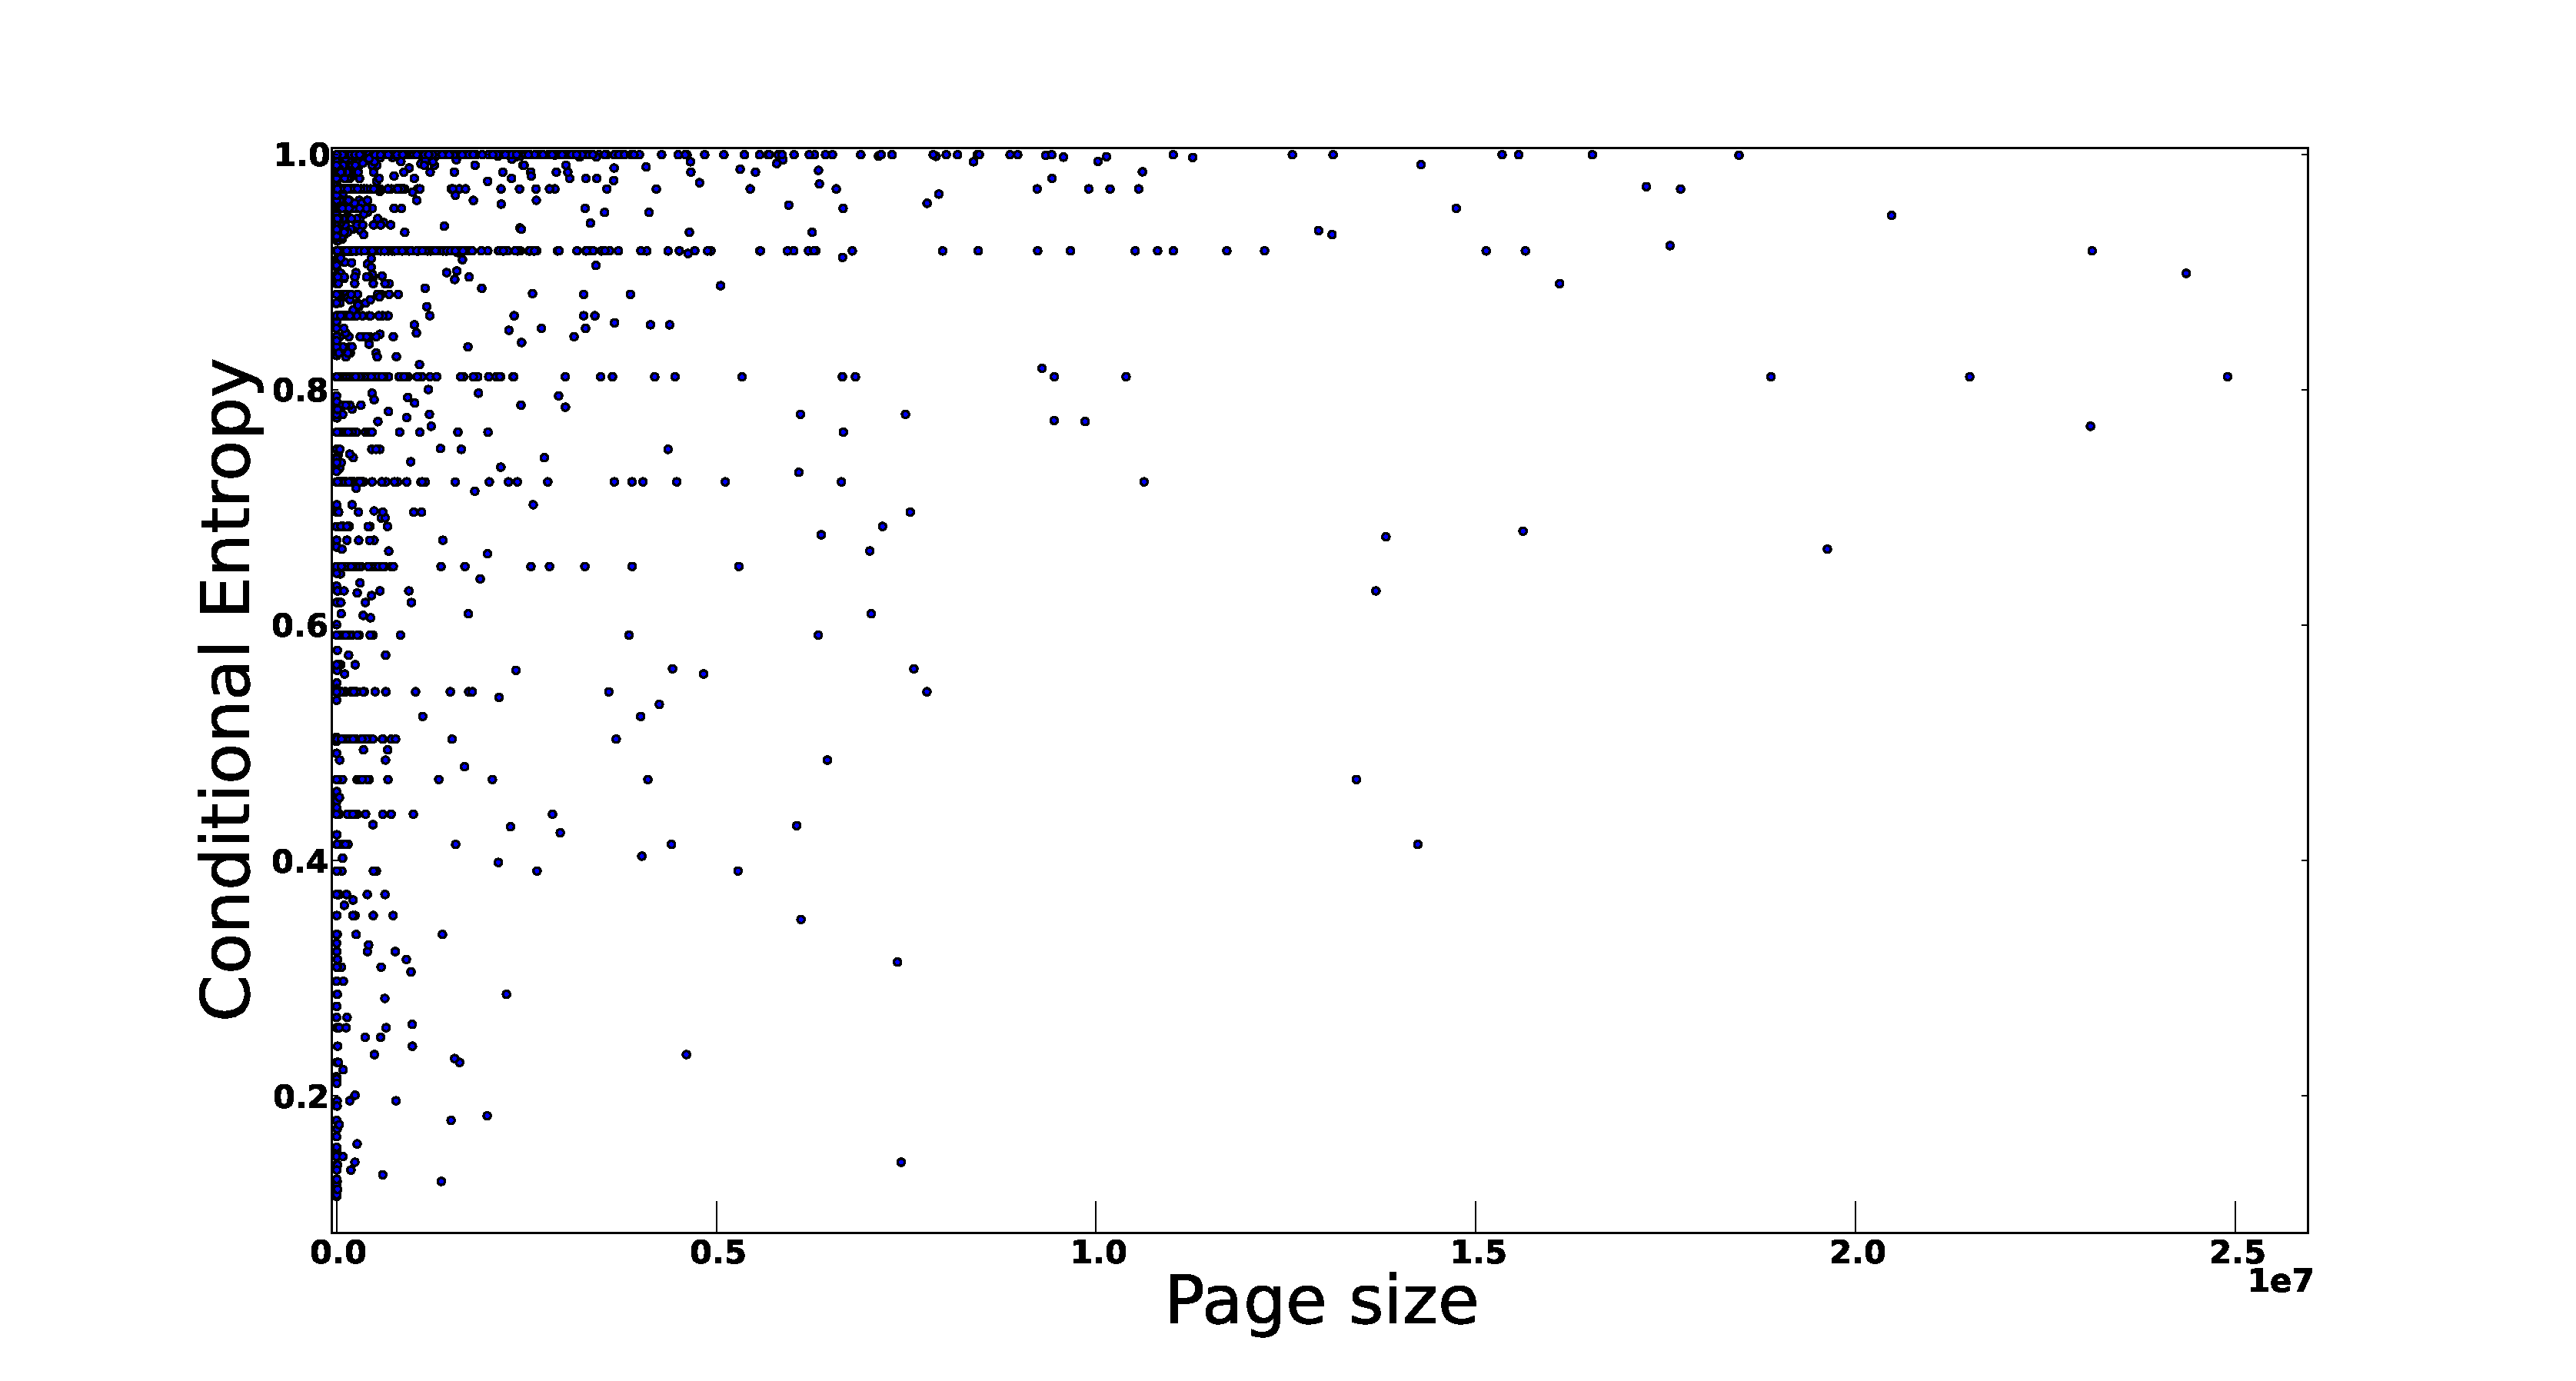
\includegraphics[width=45mm, height=35mm]{data/plots/new/CEvsPageSize.eps}}
\subfloat[Fig:][]{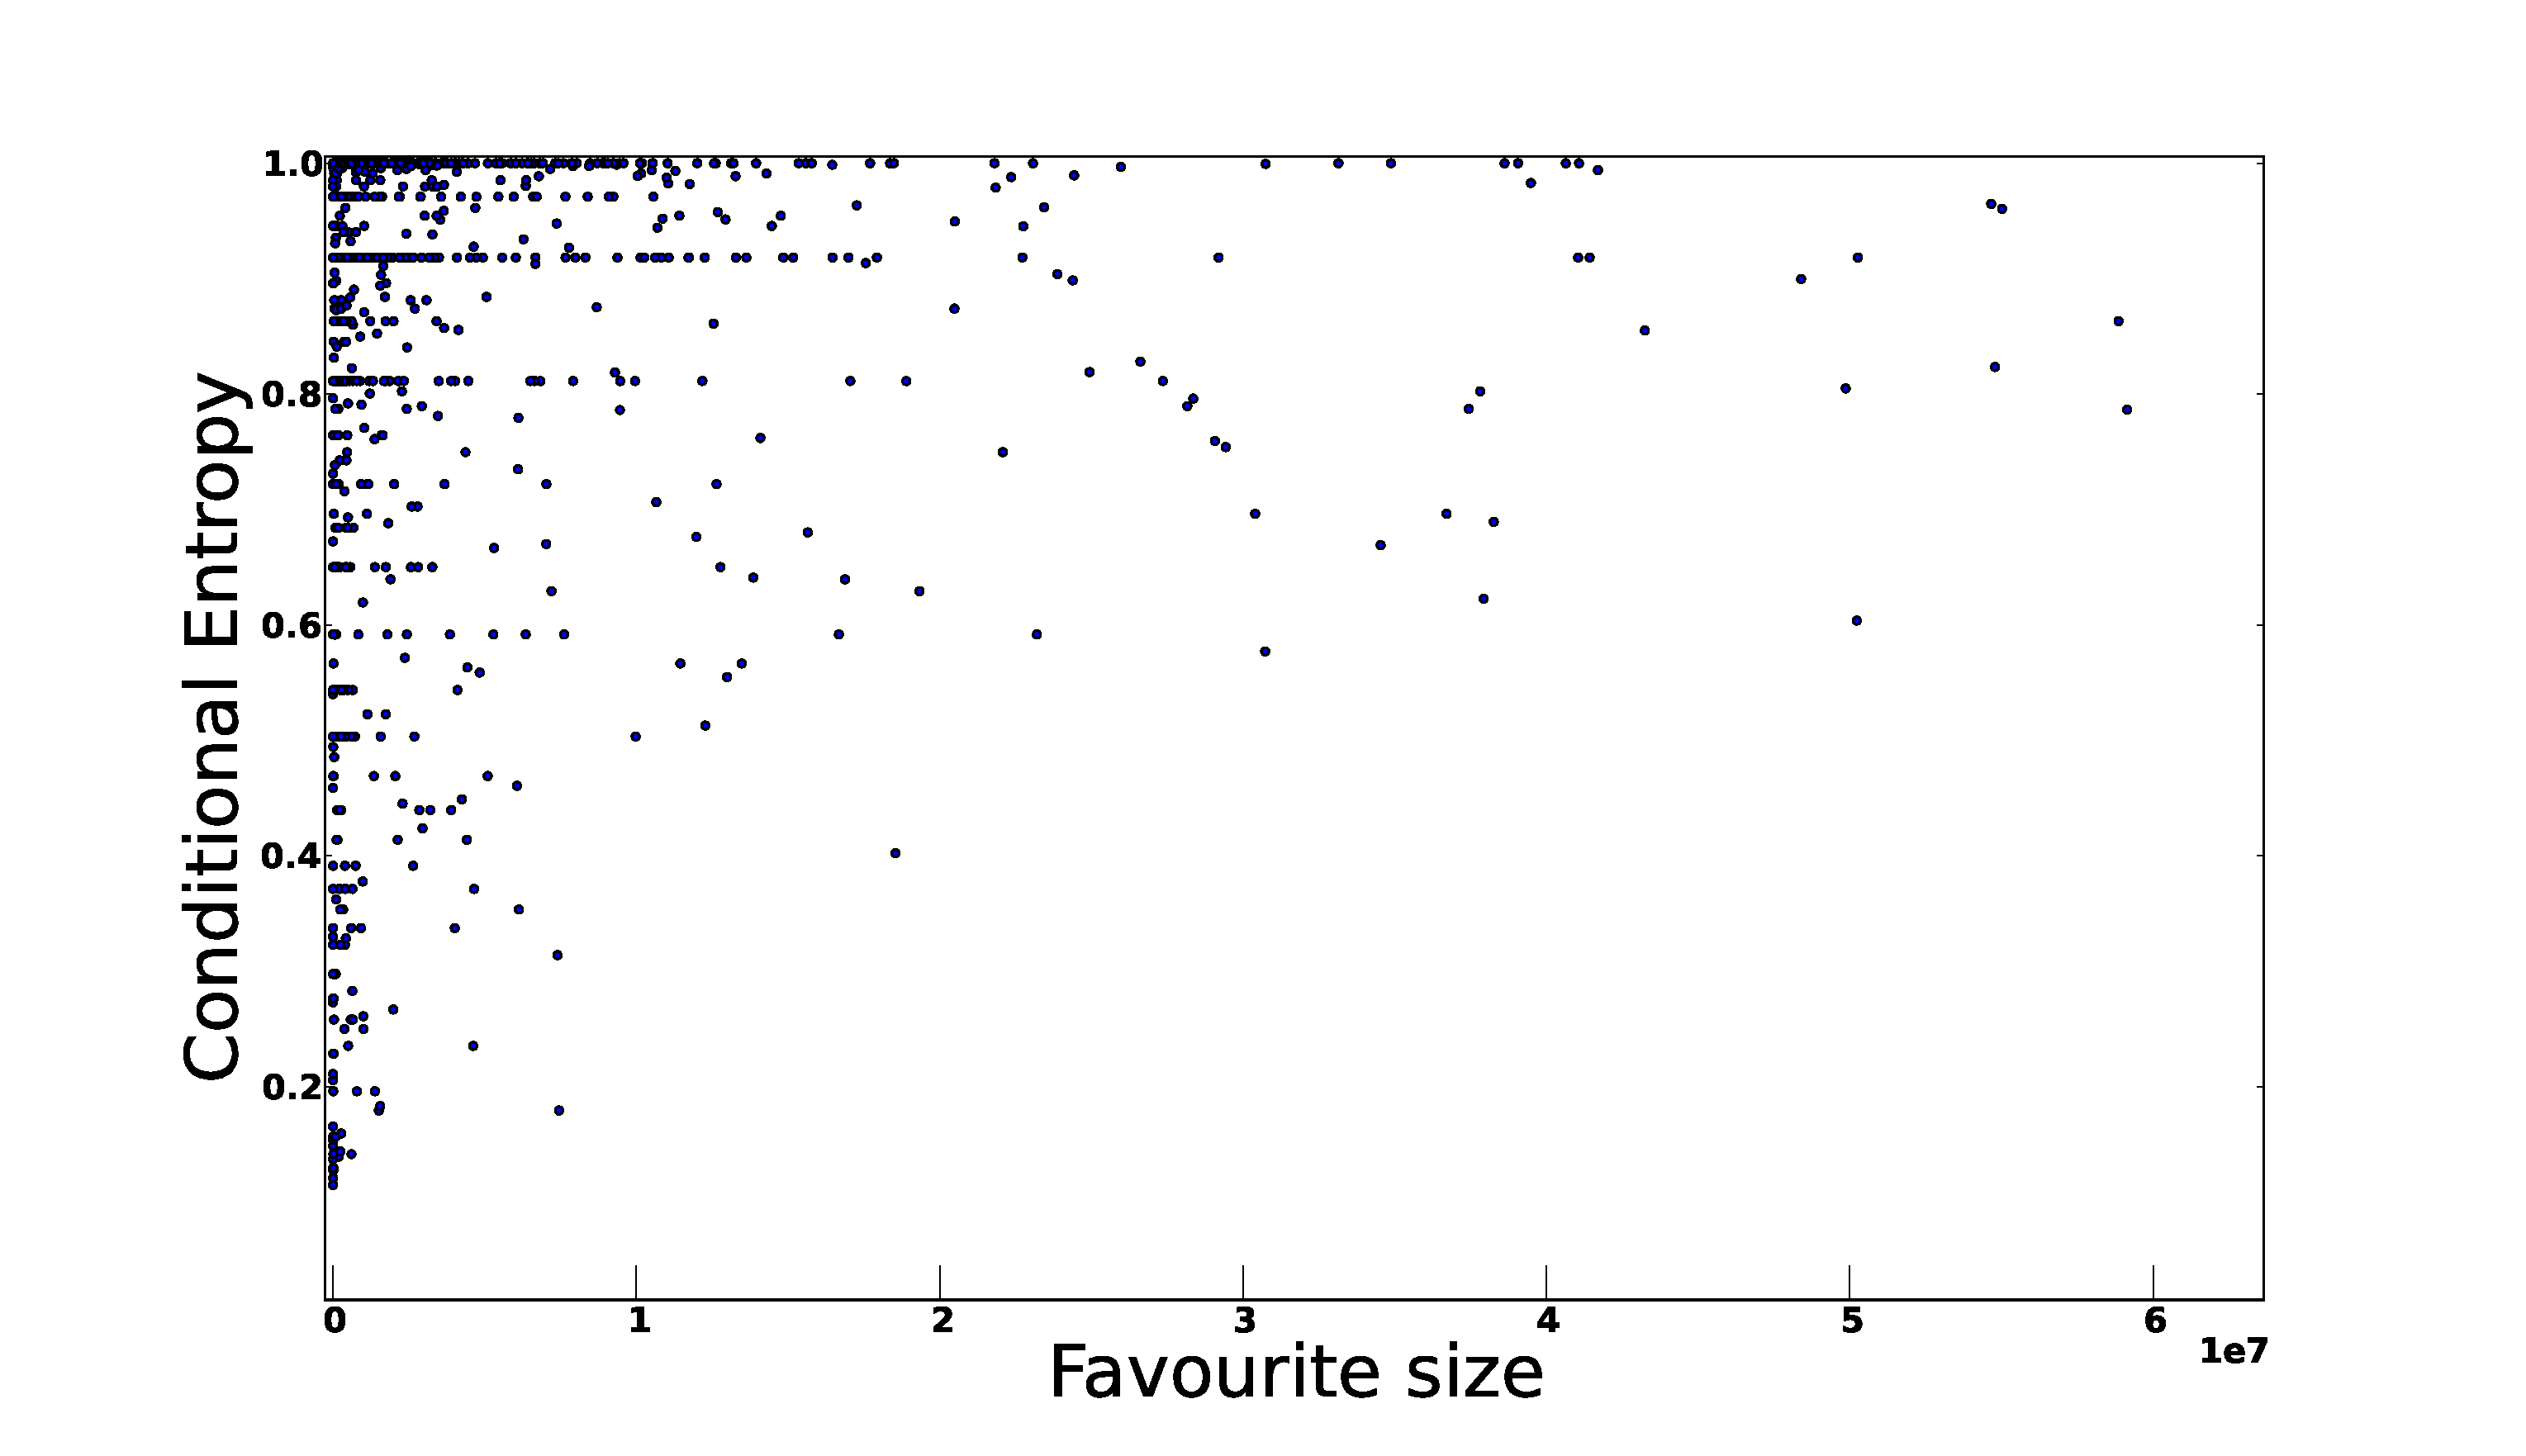
\includegraphics[width=45mm, height=35mm]{data/plots/new/CEvsFavSize.eps}} \\
%\vspace{-10mm}
\subfloat[Fig:][]{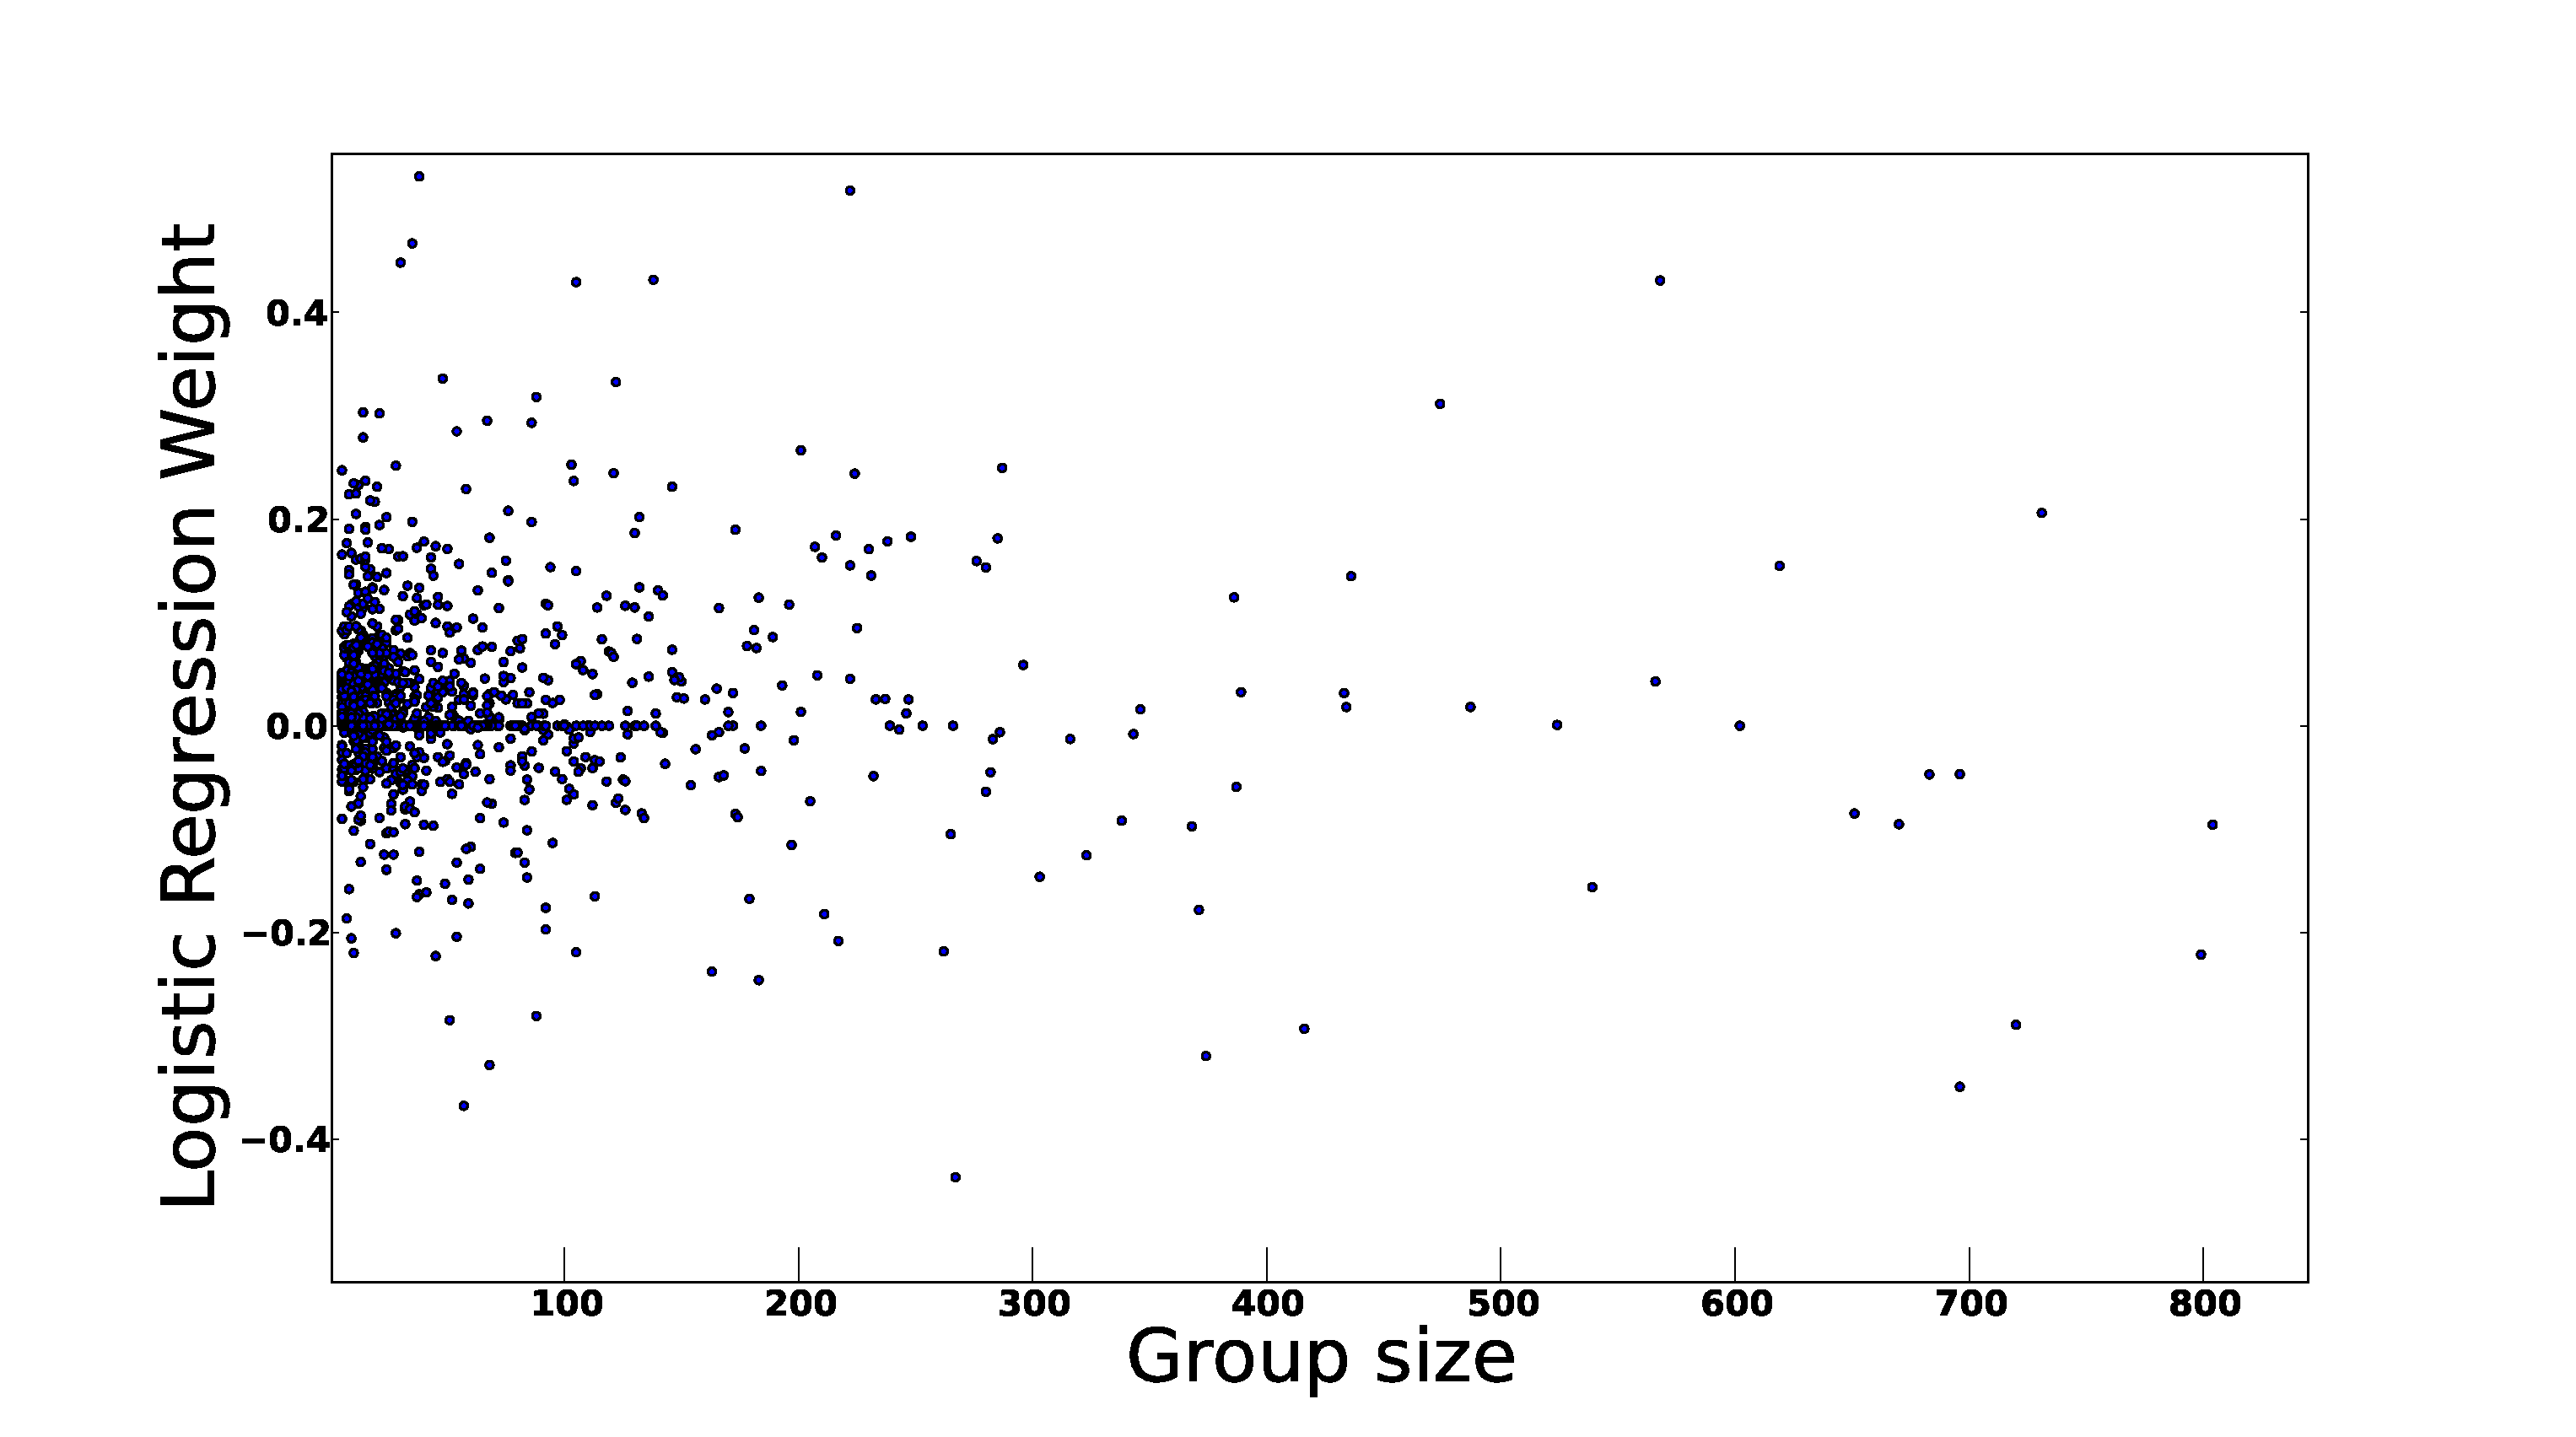
\includegraphics[width=45mm, height=35mm]{data/plots/new/LRweightvsGroupSize.eps}}
\subfloat[Fig:][]{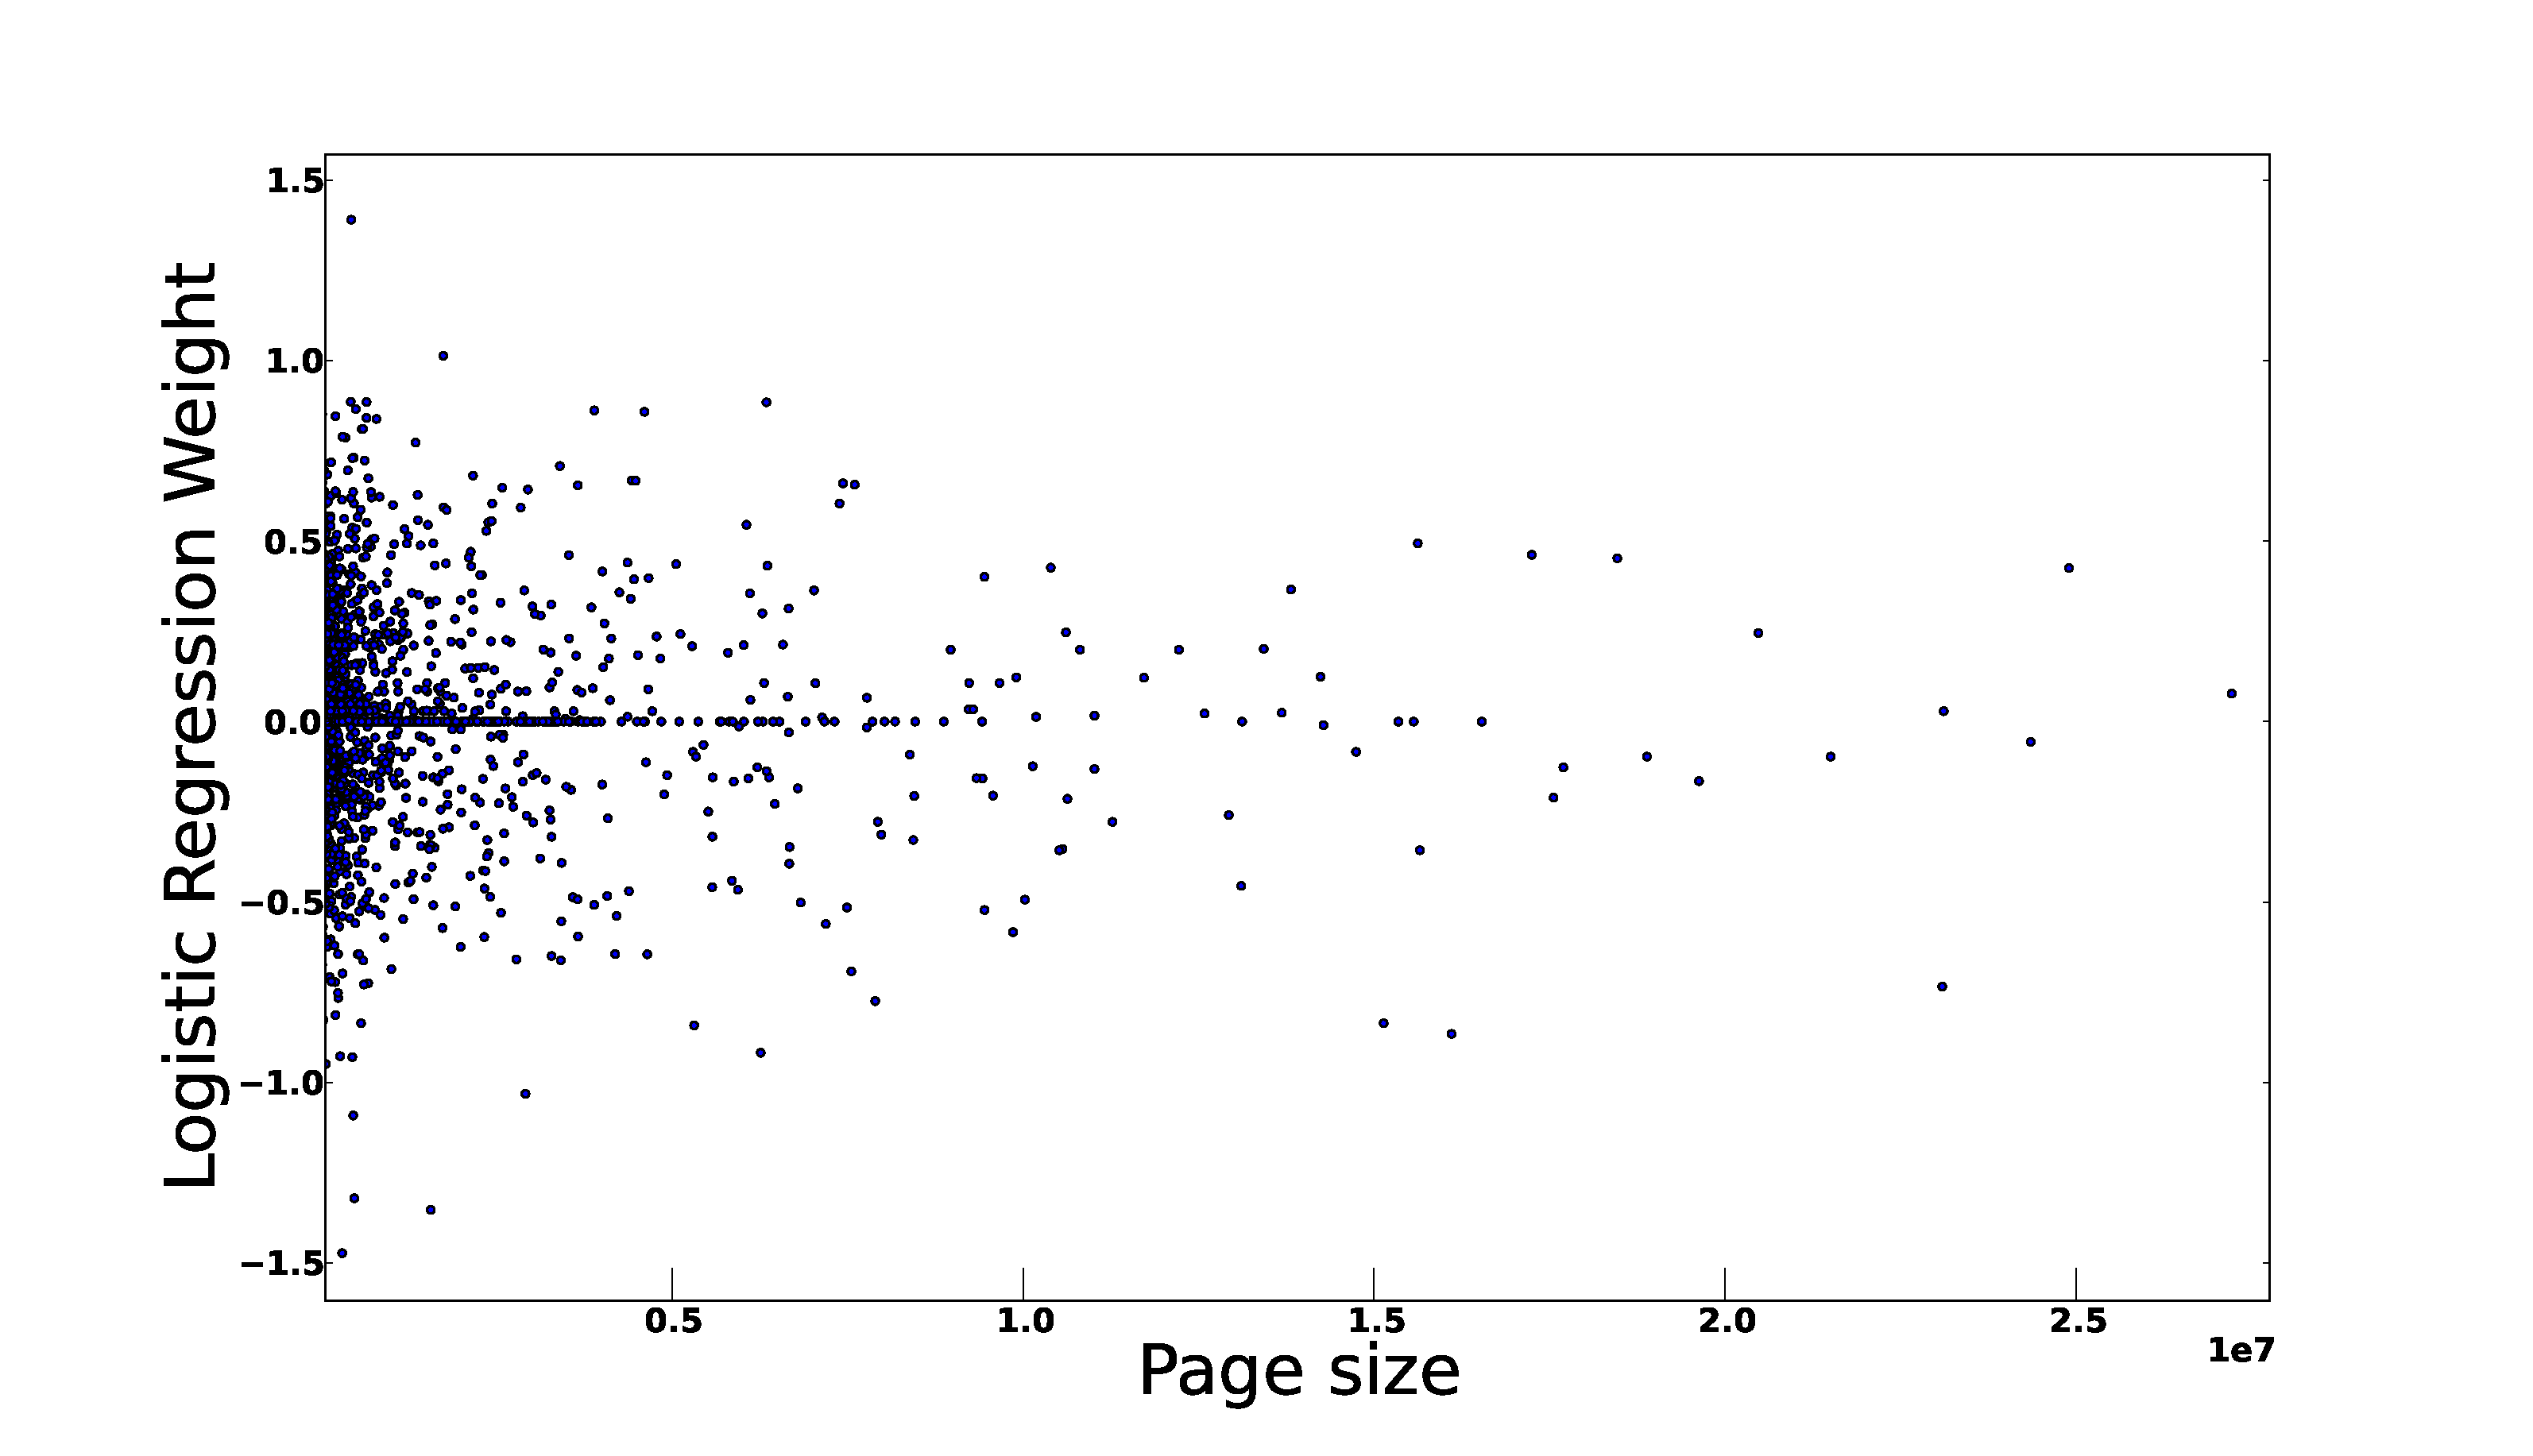
\includegraphics[width=45mm, height=35mm]{data/plots/new/LRweightvsPageSize.eps}}
\subfloat[Fig:][]{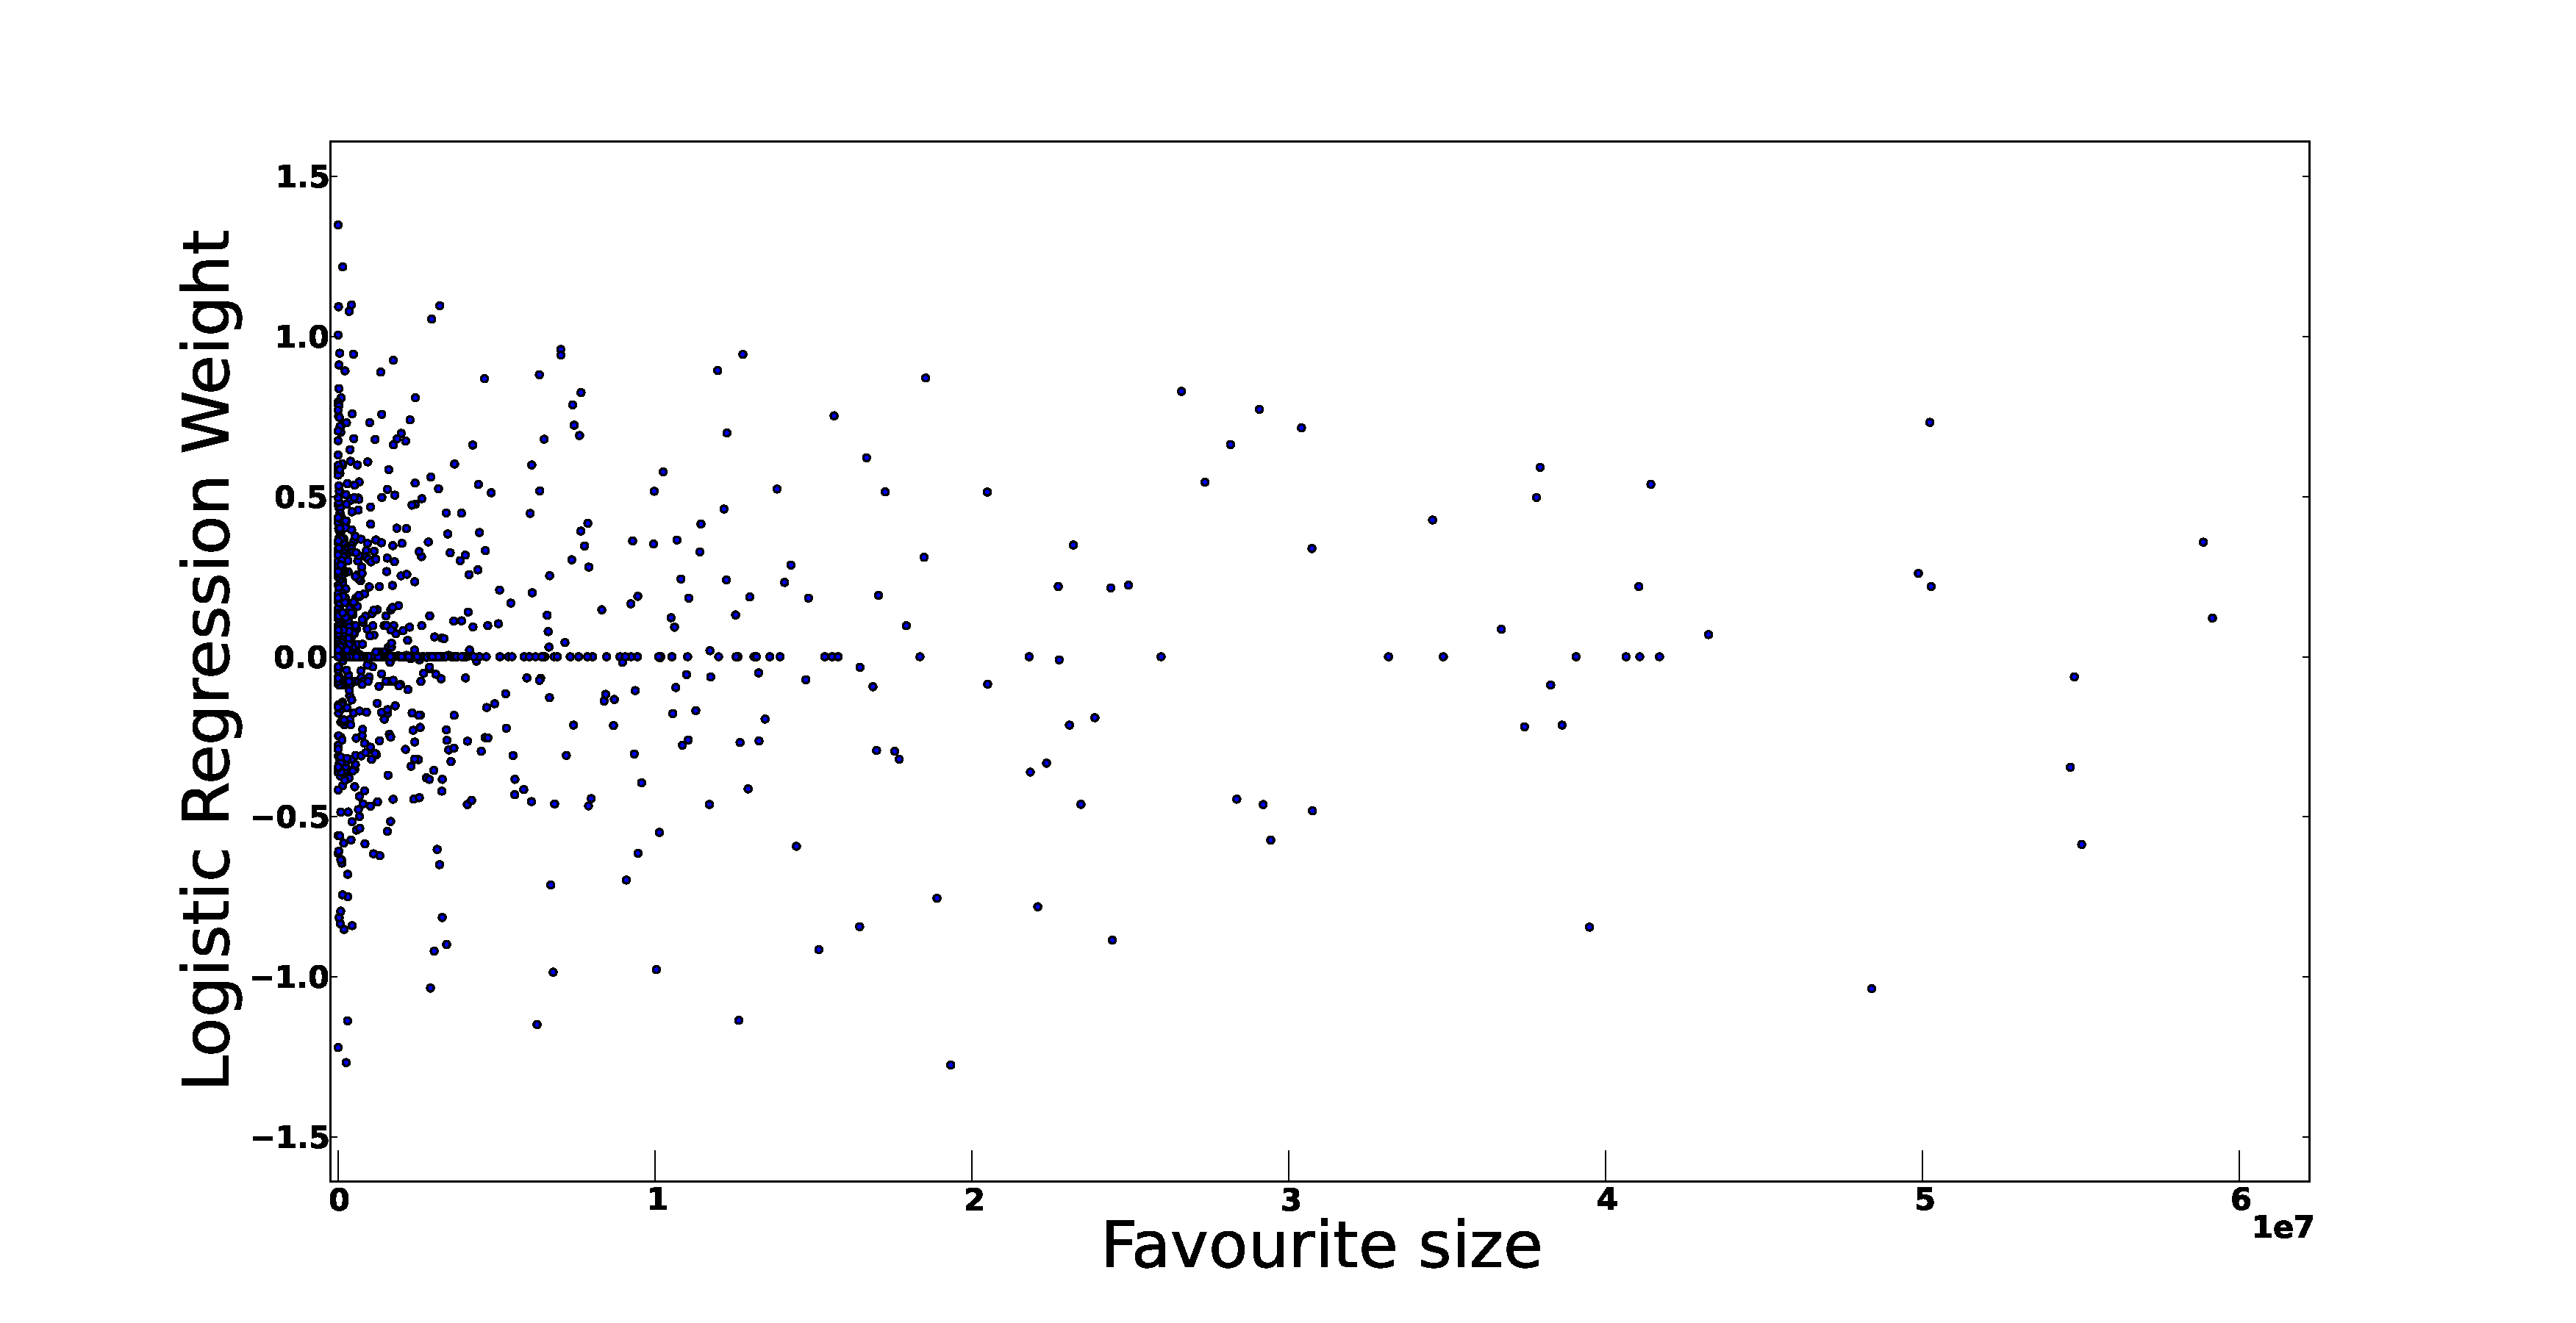
\includegraphics[width=45mm, height=35mm]{data/plots/new/LRweightvsFavSize.eps}} \\
\end{tabular}
\end{tabular}
\vspace{-2mm}
\caption {Conditional entropy vs size (a-c); logistic regression feature weights vs size (d-f).
In (a-c) we observe that the large membership ASAGs are rarely informative while the most
informative SAGs tend to have low memberships.  Similarly in (d-f) we see that the most
predictive features with the most extreme weights are concentrated toward small ASAGs. }
\label{Fig3}
\end{figure*}
%%%%%%%%%%%%%%%%%%%%%%%%%%%%%%%%%%%%%%%%%%%%%%%%%%%%%%%%%%%%%%%%%%%%%%%%%%%

%\vspace{-5mm}

%%%%%%%%%%%%%%%%%%%%%%%%%%%%%%%%%%%%%%%%%%%%%%%%%%%%%%%%%%%%%%%%%%%%%%%%%%%
\begin{figure*}[tbp!]
\centering
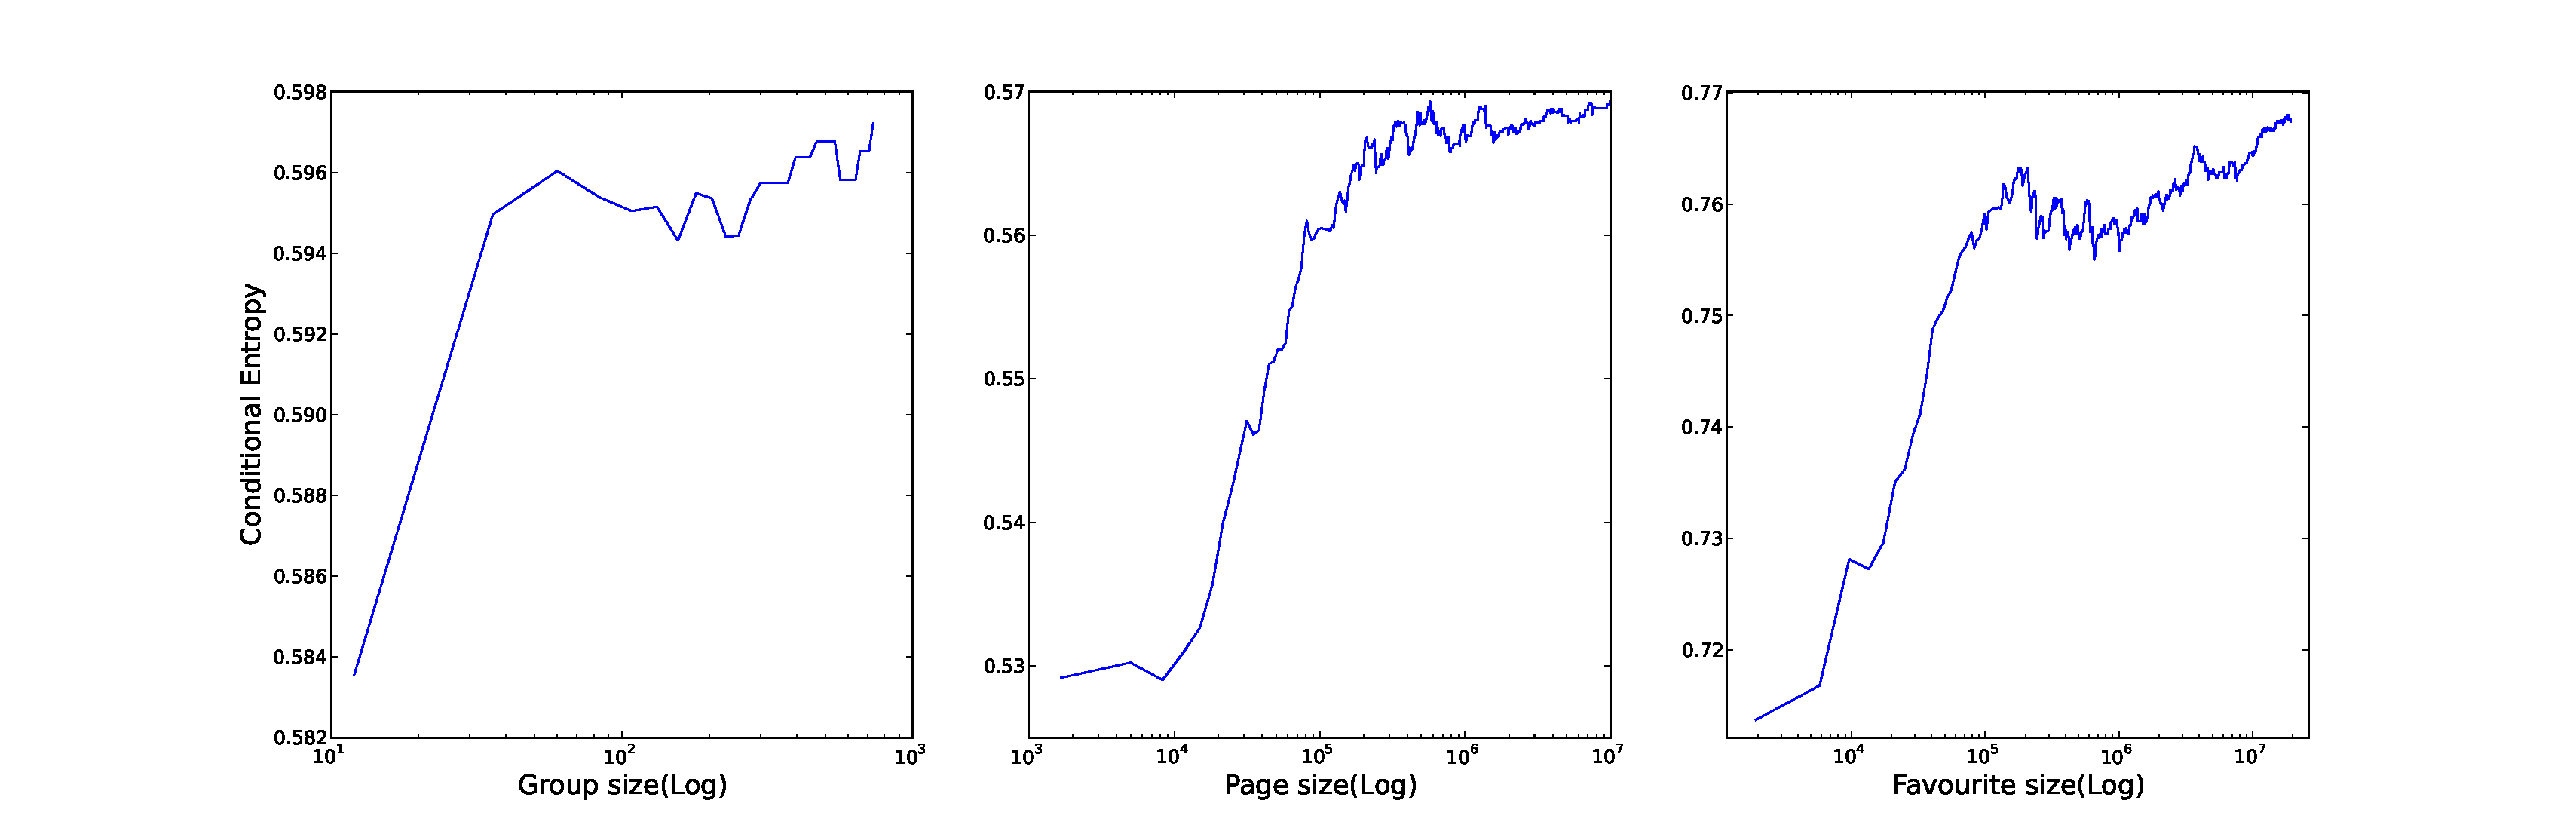
\includegraphics[scale=0.28]{data/plots/cumulativeEntropy/cumulative.eps}
\vspace{-3mm}
\caption{Average conditional entropy of top 10\% groups, pages and favourite features \emph{cumulative} over the size.  Here we see that as we add in larger membership ASAGs, the average informativeness
decreases substantially (entropy increases).}
\label{Fig4}
\end{figure*}
%%%%%%%%%%%%%%%%%%%%%%%%%%%%%%%%%%%%%%%%%%%%%%%%%%%%%%%%%%%%%%%%%%%%%%%%%%%

%\vspace{-7mm}

%%%%%%%%%%%%%%%%%%%%%%%%%%%%%%%%%%%%%%%%%%%%%%%%%%%%%%%%%%%%%%%%%%%%%%%%%%%
\begin{figure*}[tbp!]
\hspace{-12mm}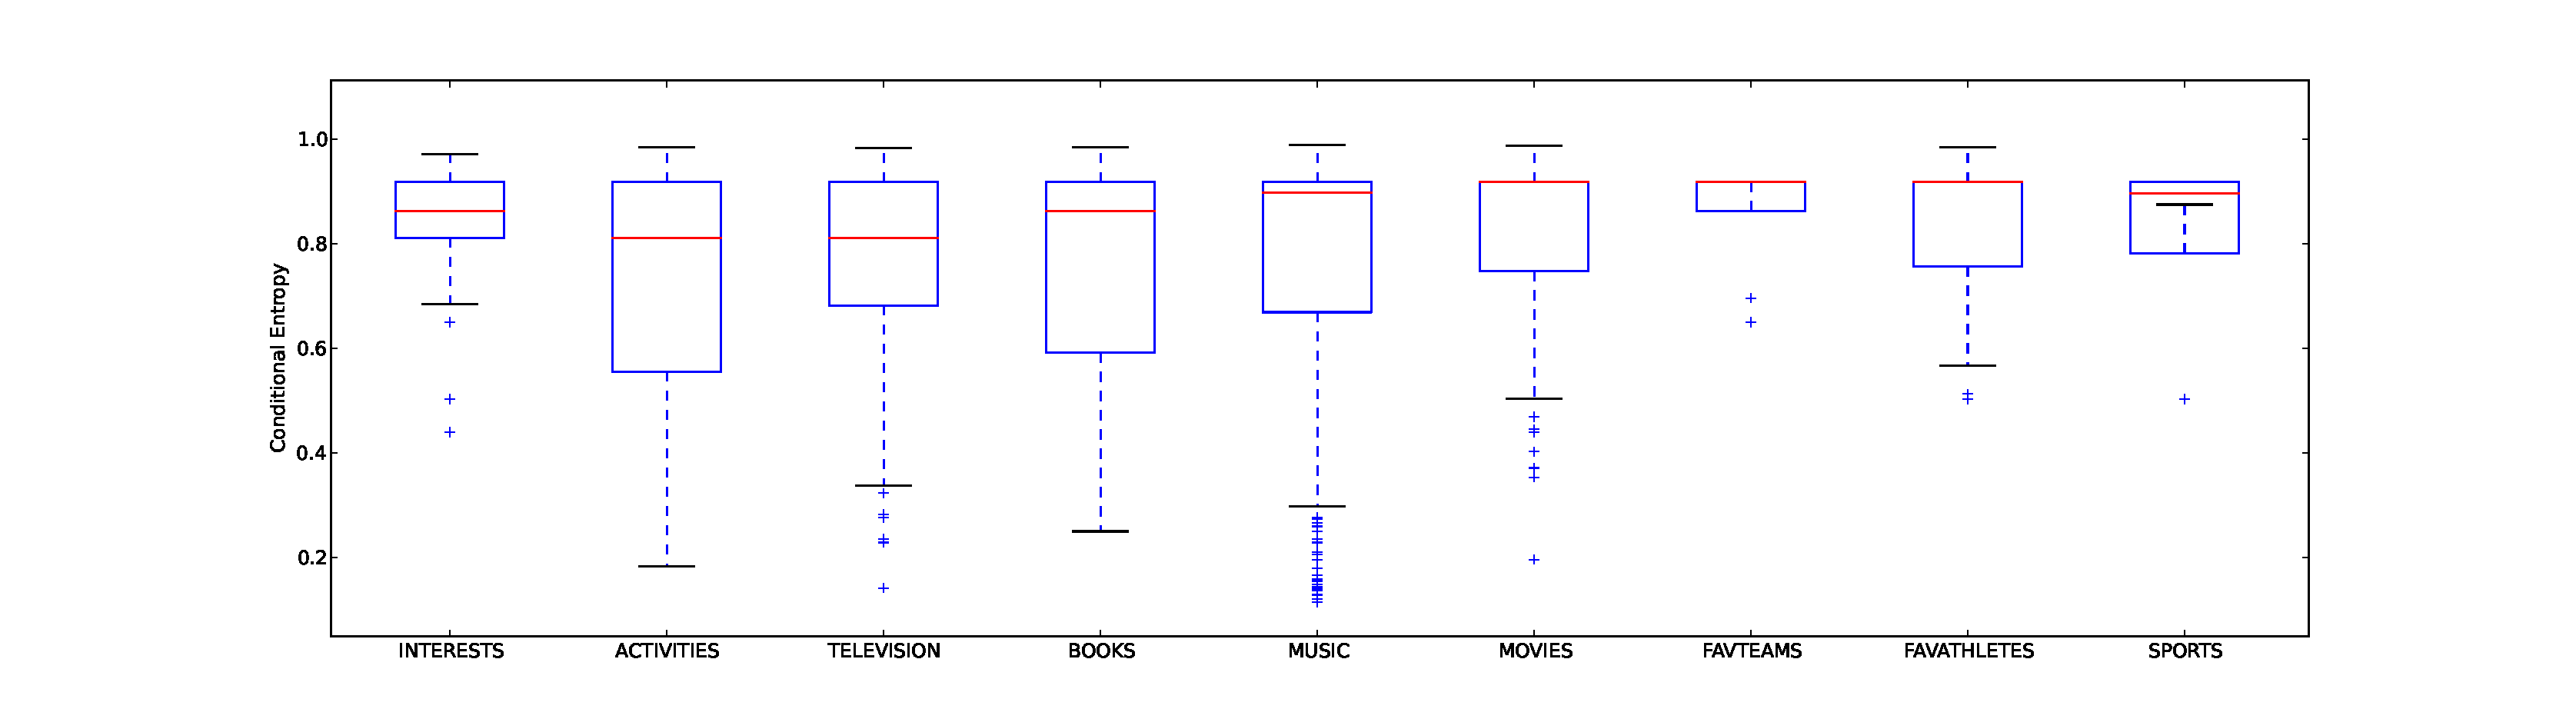
\includegraphics[width=200mm]{data/plots/boxPlots/CEvsFavTypes.eps}
\vspace{-7mm}
\caption{Conditional entropy for top 1000 favourites breakdown by categories.  While ASAG categories
with many options like music are not informative on average, we see
that some of the most informative ASAGs are music.  This reiterates
the point that it is crucial to \emph{learn} which ASAGs (or ISAGs)
are informative rather than aggregating average information.}
\label{Fig5}
\end{figure*}
%%%%%%%%%%%%%%%%%%%%%%%%%%%%%%%%%%%%%%%%%%%%%%%%%%%%%%%%%%%%%%%%%%%%%%%%%%%

%#suvash#
\begin{figure*}[tbh!]
\centering
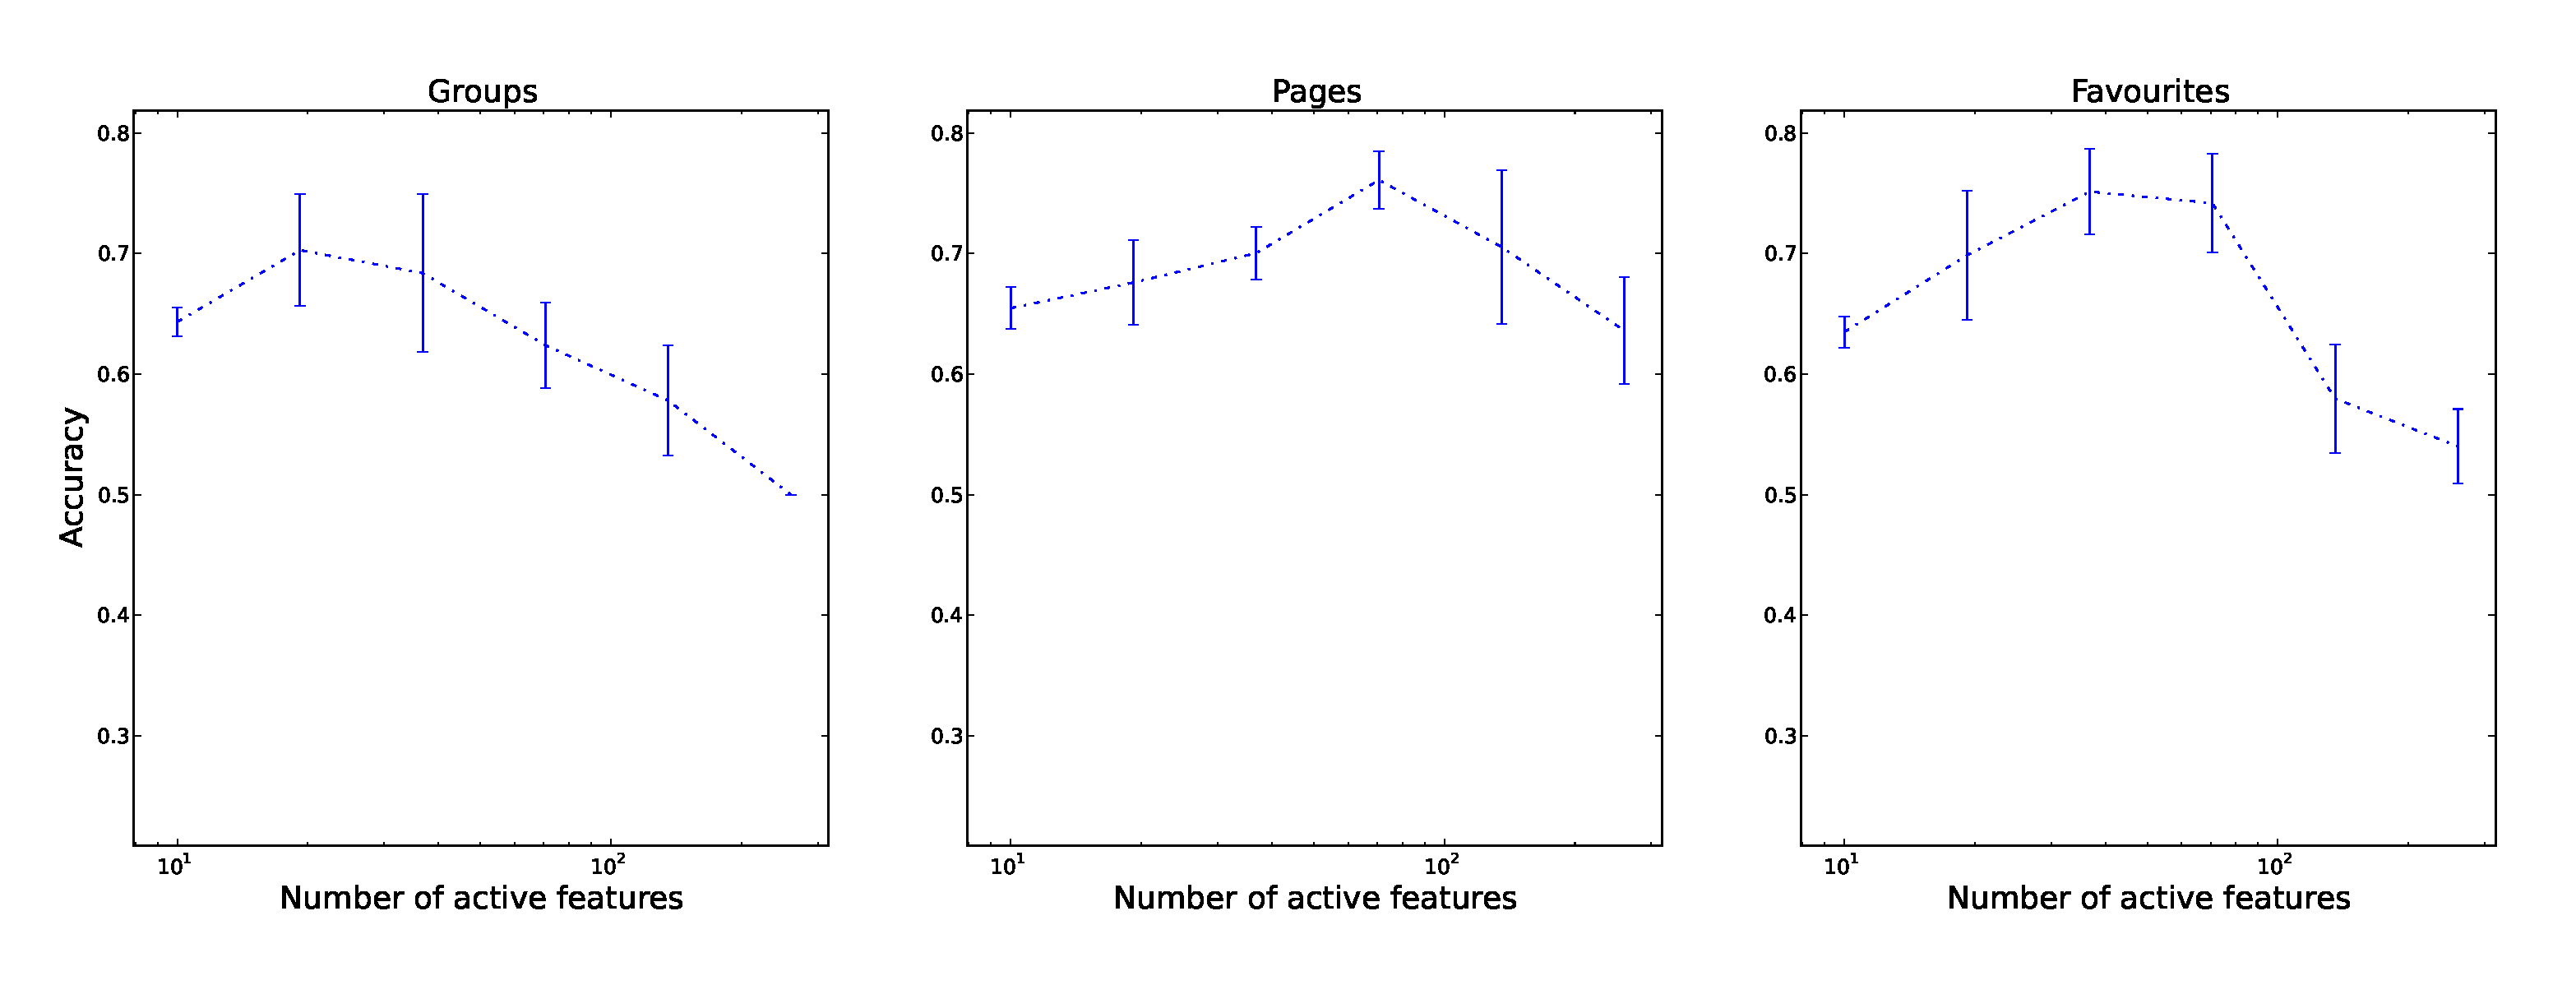
\includegraphics[width=180mm, height=50mm]{data/plots/new/accuracyVsactiveFeatures.eps}
\vspace{-6mm}
\caption{Accuracy increases as the number of active features increases, but then, after reaching a certain limit, it starts to decrease sharply.
}
\label{fig:AccuracyVsactiveFeats}
\end{figure*}

\begin{figure*}[tbh!]
\centering
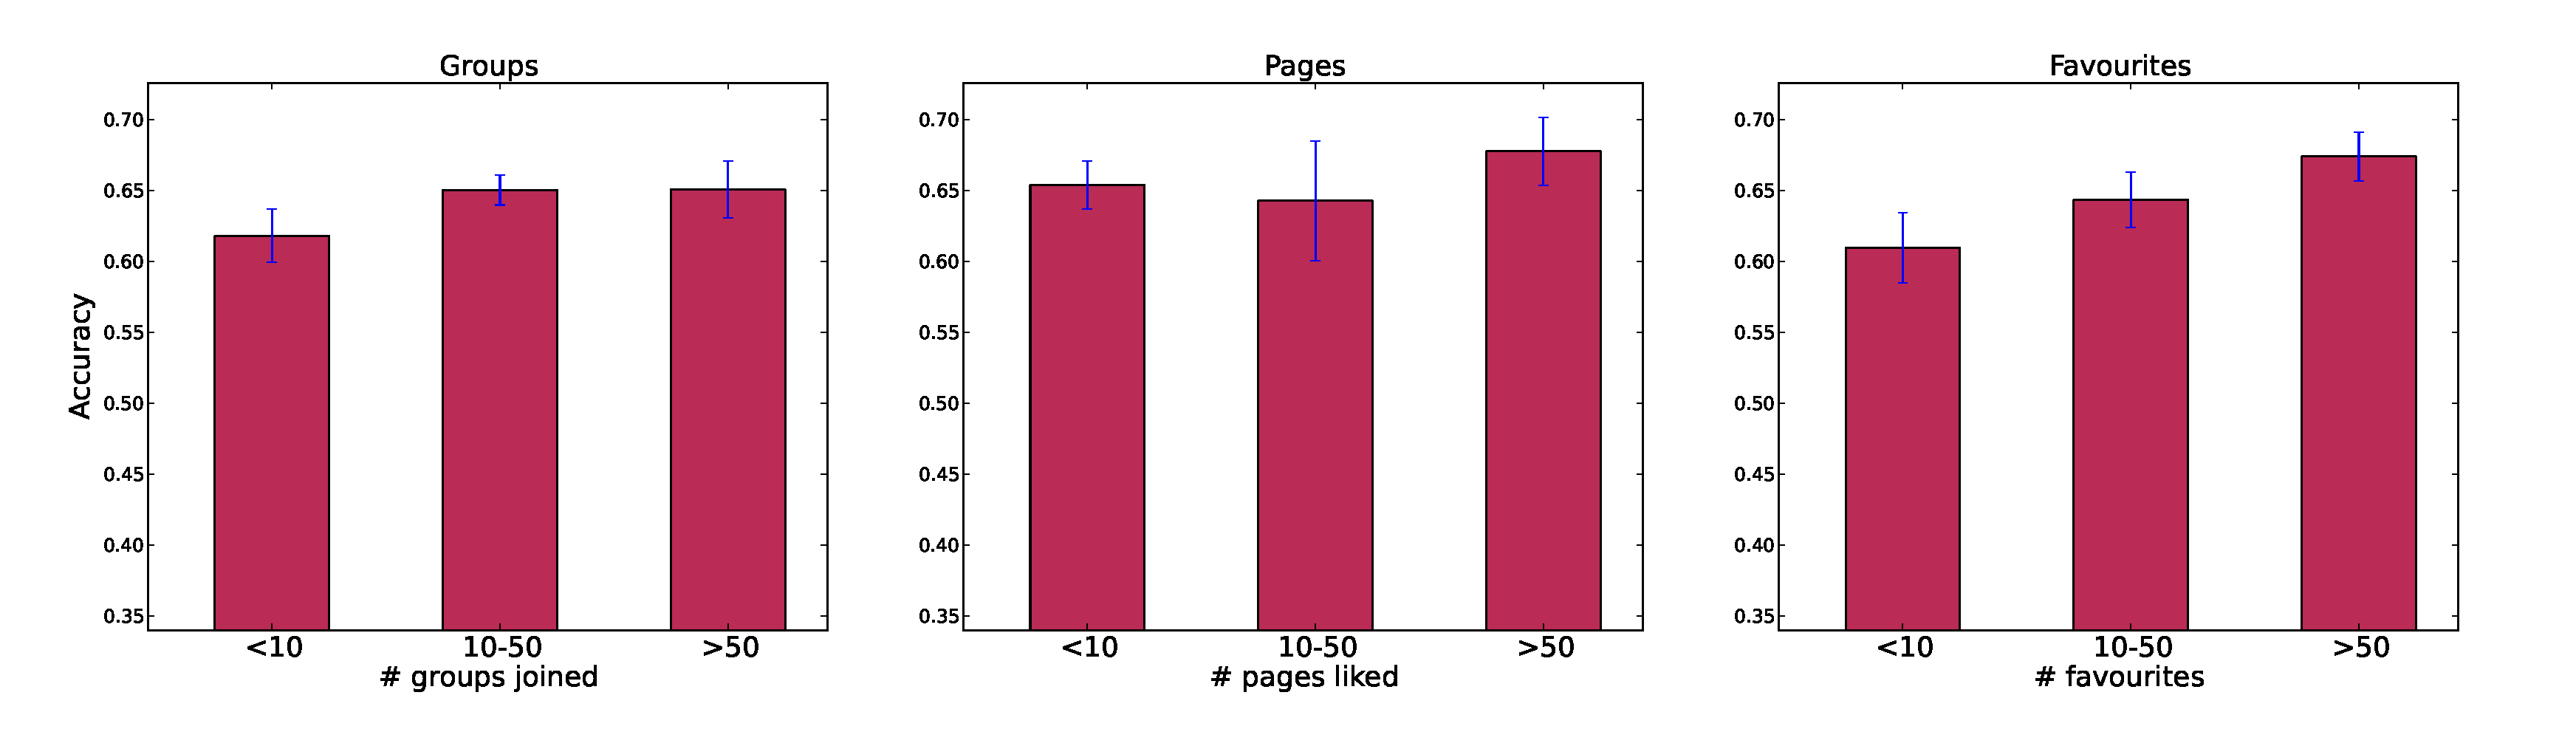
\includegraphics[width=180mm, height=50mm]{data/plots/new/accuracyVsmembership.eps}
\vspace{-6mm}
\caption{Accuracy of the SAF increases as user becomes more active in social network by joining more groups/pages/favourites.}
\label{AccuracyVsmembership}
\end{figure*}

